% ==============================================================================
% LAB 119
% UNDERSÖKNING AV RC-KRETS
% ------------------------
%
% Author:
% Jonas Sjöberg     <tel12jsg@student.hig.se>
% Oscar Wallberg    <tco13owg@student.hig.se>
%
% License:
% Creative Commons Attribution-NonCommercial-ShareAlike 4.0 International
% See LICENSE.md for full licensing information.
% ==============================================================================

\section{Appendix}\label{appendix}
% ------------------------------------------------------------------------------

\subsection{Signalgenerator}
De värden som presenteras i rapporten uppmättes med ett analogt 2-kanals
oscilloskop \texttt{Hitachi V-252} med en bandbredd på \SI{20}{\MHz}.  Signalen
genererades av en hemmabyggd egendesignad signalgenerator.  Kopplingsschema
till signalgeneratorn återfinns i Figur~\ref{fig:siggen-sch}.  Stabiliteten och
precisionen hos signalgeneratorn lämnar en del att önska, likaså är
oscilloskopet inte särskilt lättanvänt. Avläsning måste ske ``manuellt'' genom
att divisionerna på oscilloskopskärmen räknas och multipliceras med vald tidbas
eller vertikal förstärkning.


%\begin{figure}[ht]\label{fig:siggen-sch1}
  %\centering
  %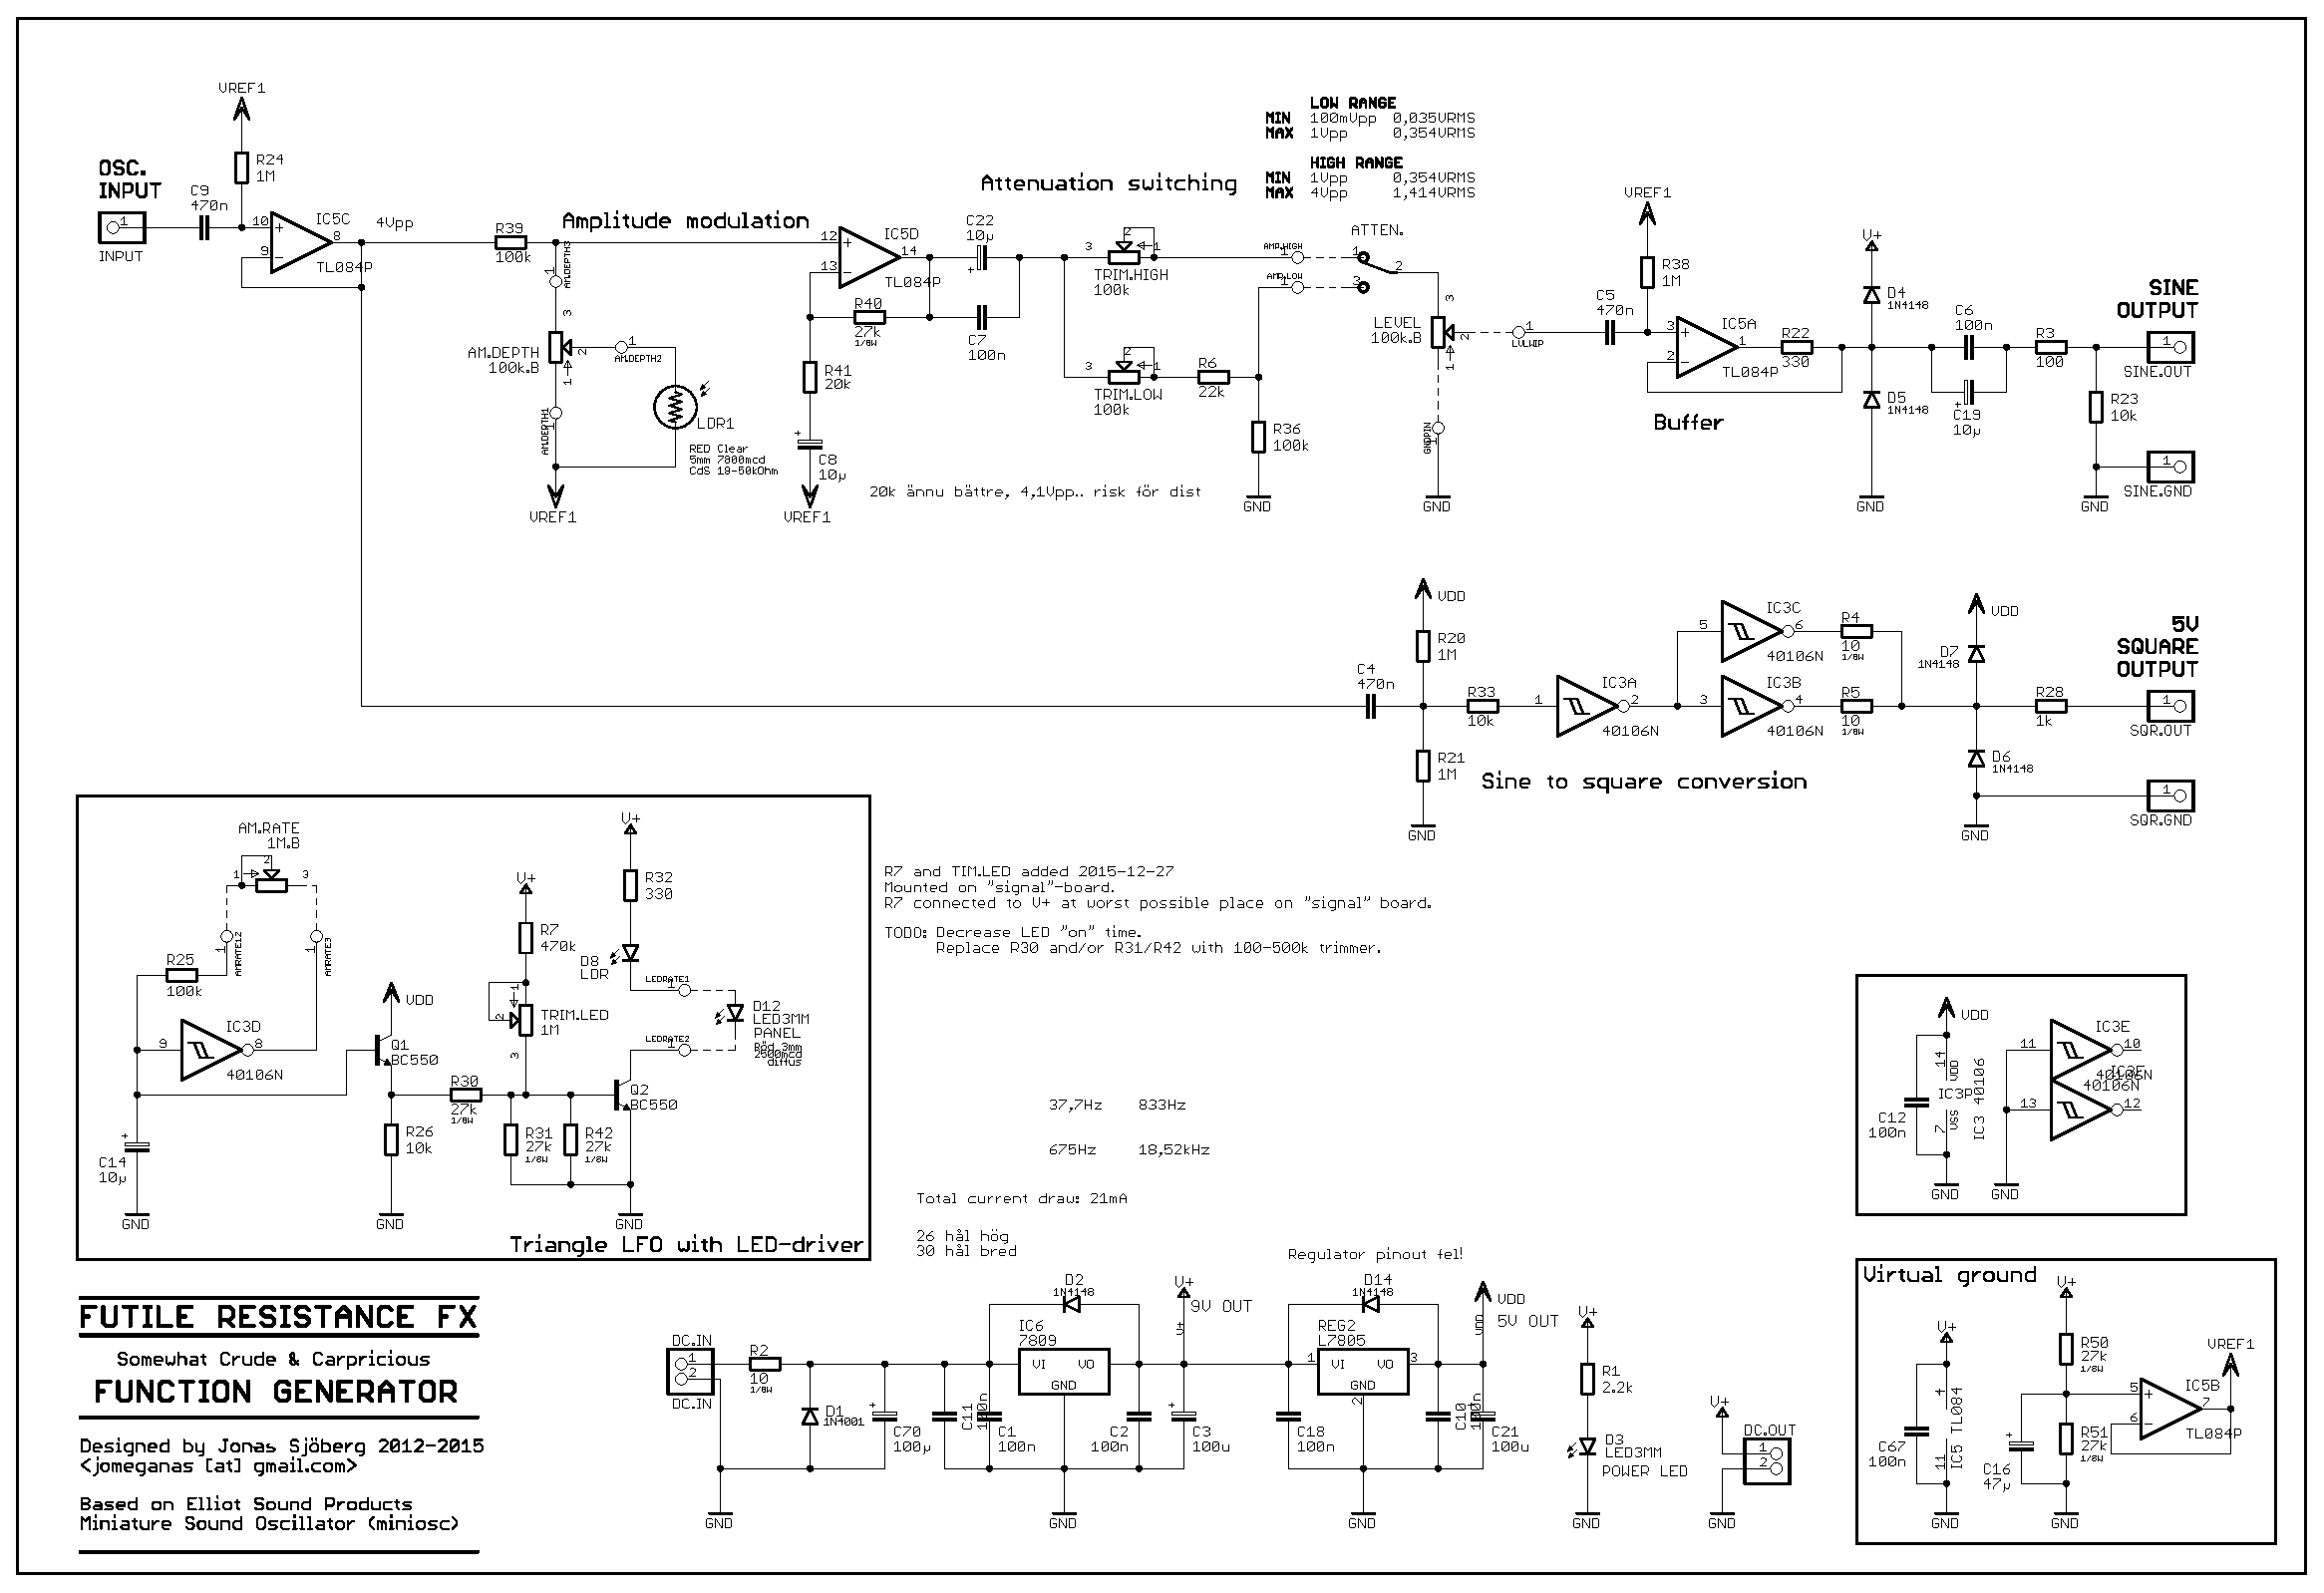
\includegraphics[width=\linewidth]{img/signal-generator_schematic-1}
  %\caption[] {Kopplingsschema för signalgeneratorn som användes vid laborationen.}
%\end{figure}

%\begin{figure}[ht]\label{fig:siggen-sch2}
  %\centering
  %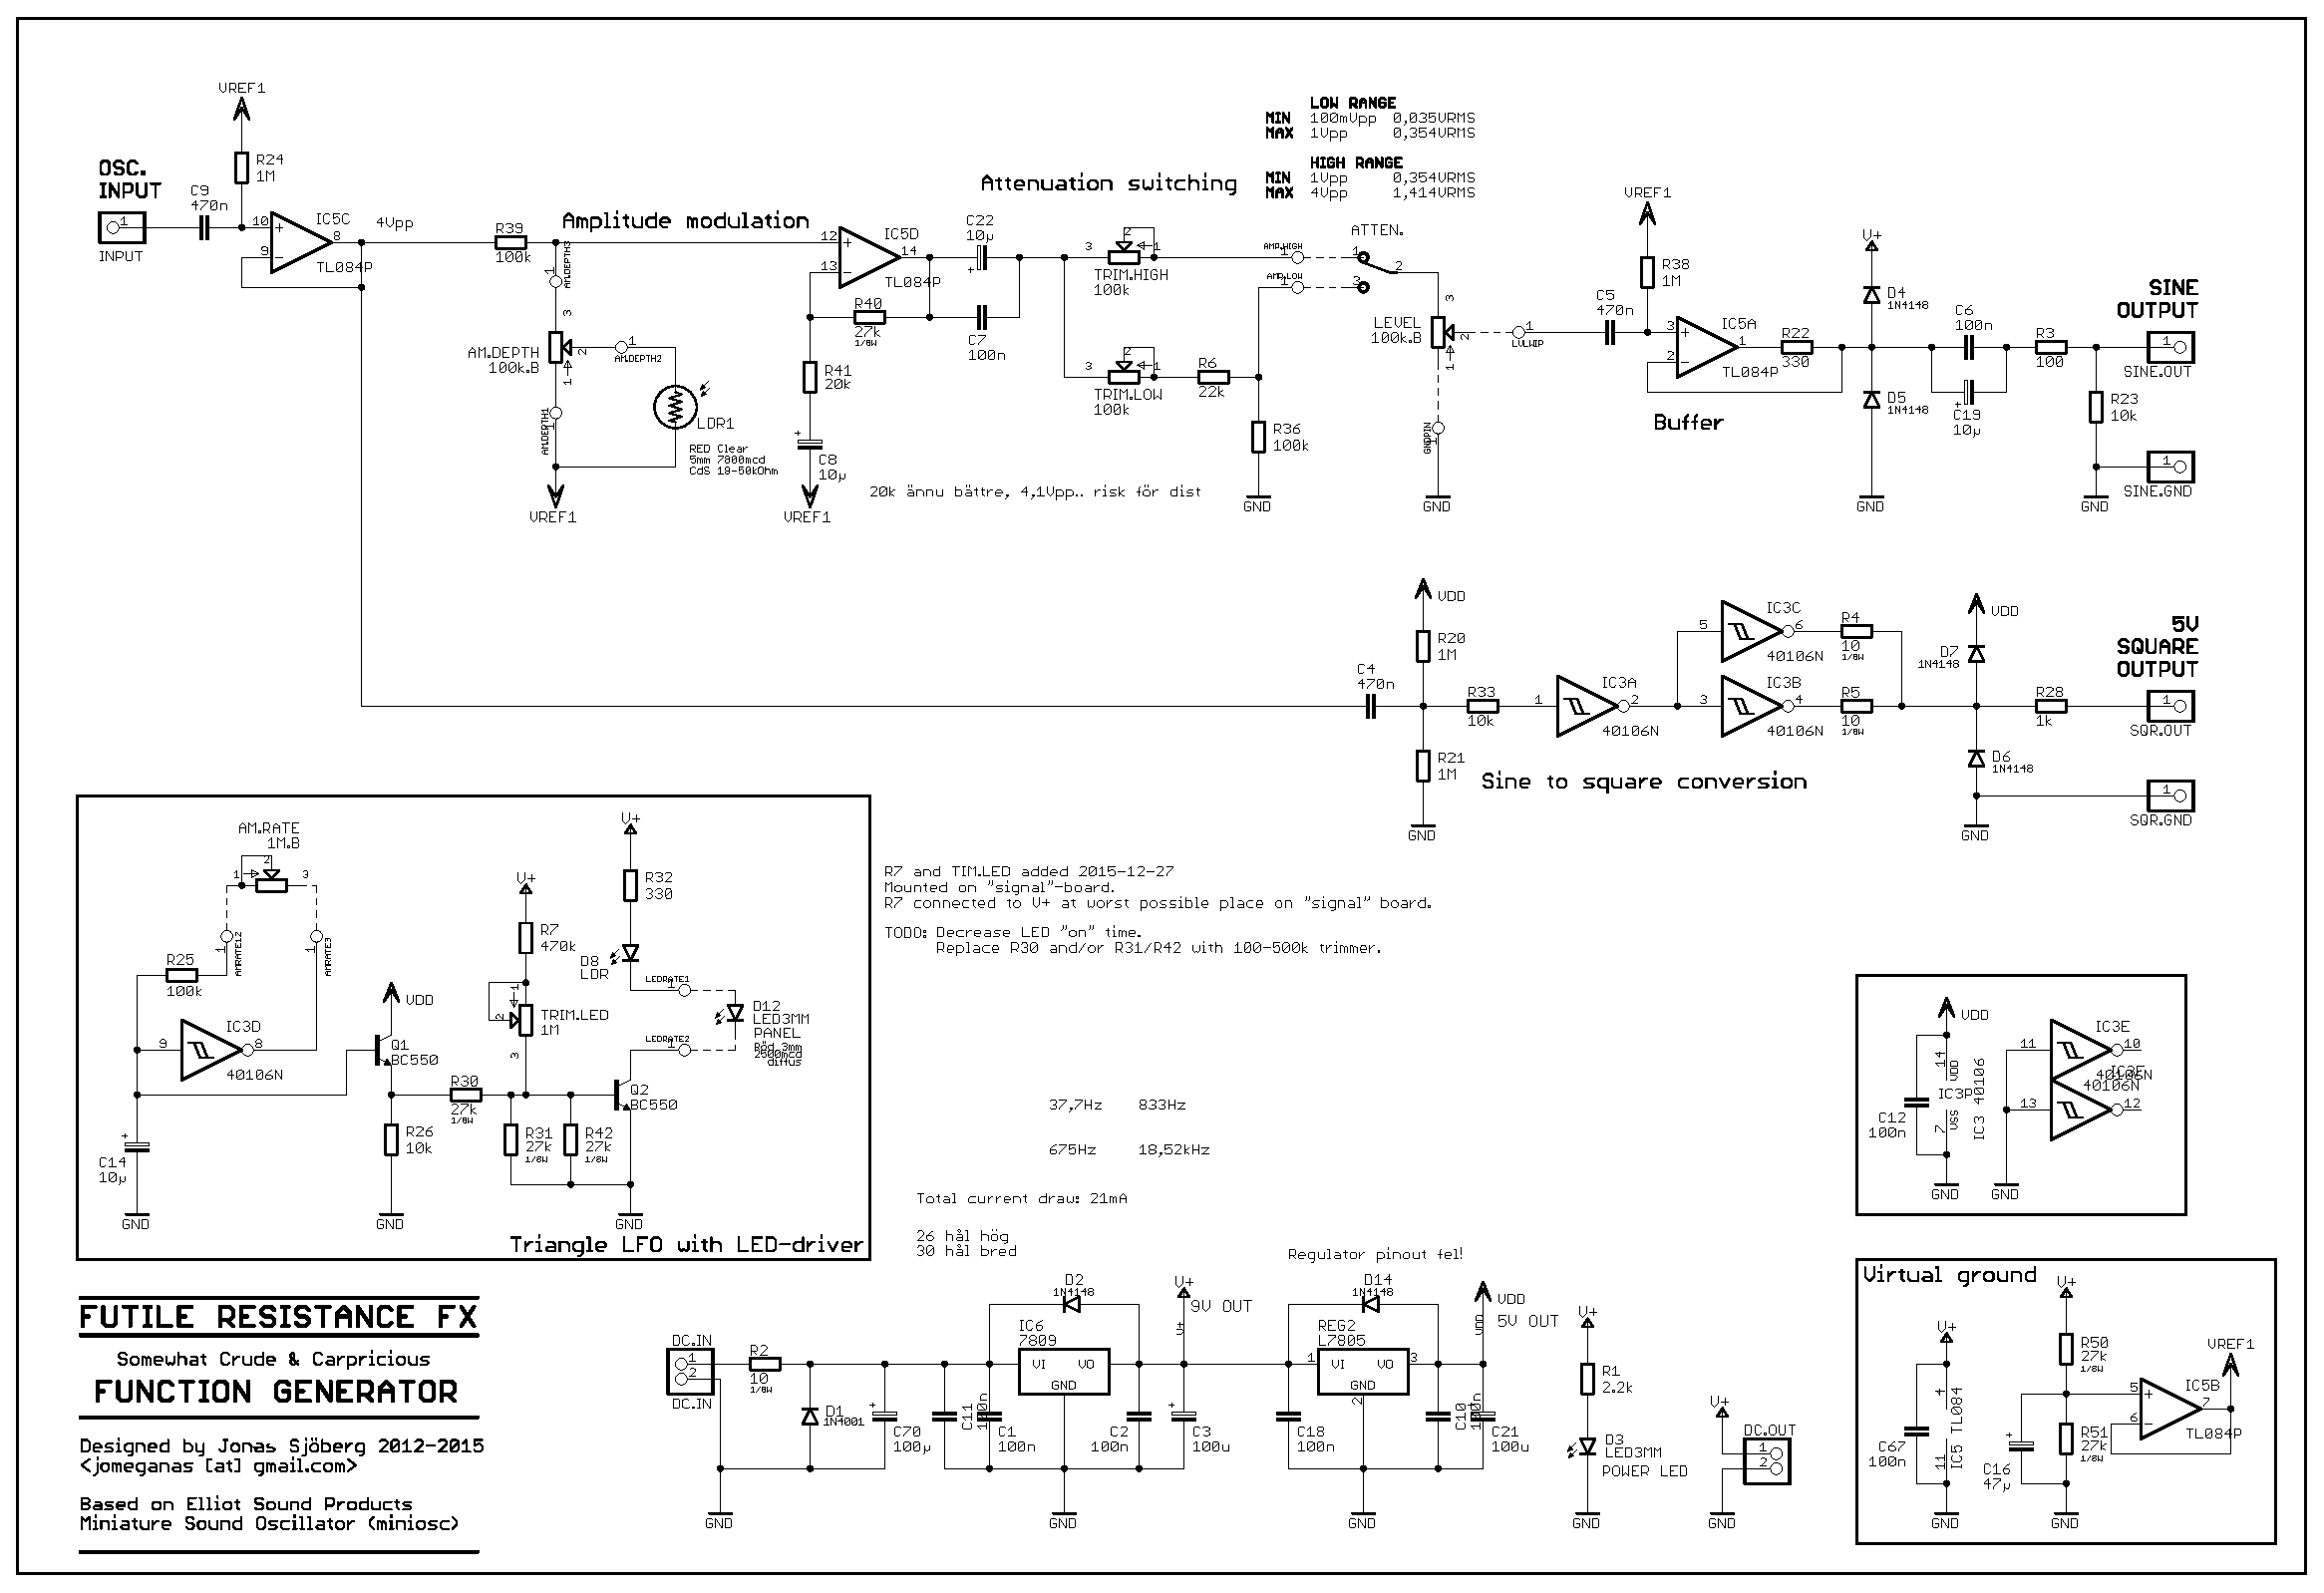
\includegraphics[width=\linewidth]{img/signal-generator_schematic-1}
  %\caption[] {Kopplingsschema för signalgeneratorn som användes vid laborationen.}
%\end{figure}

\begin{sidewaysfigure}[ht]\label{fig:siggen-schem-1}
 \centering
 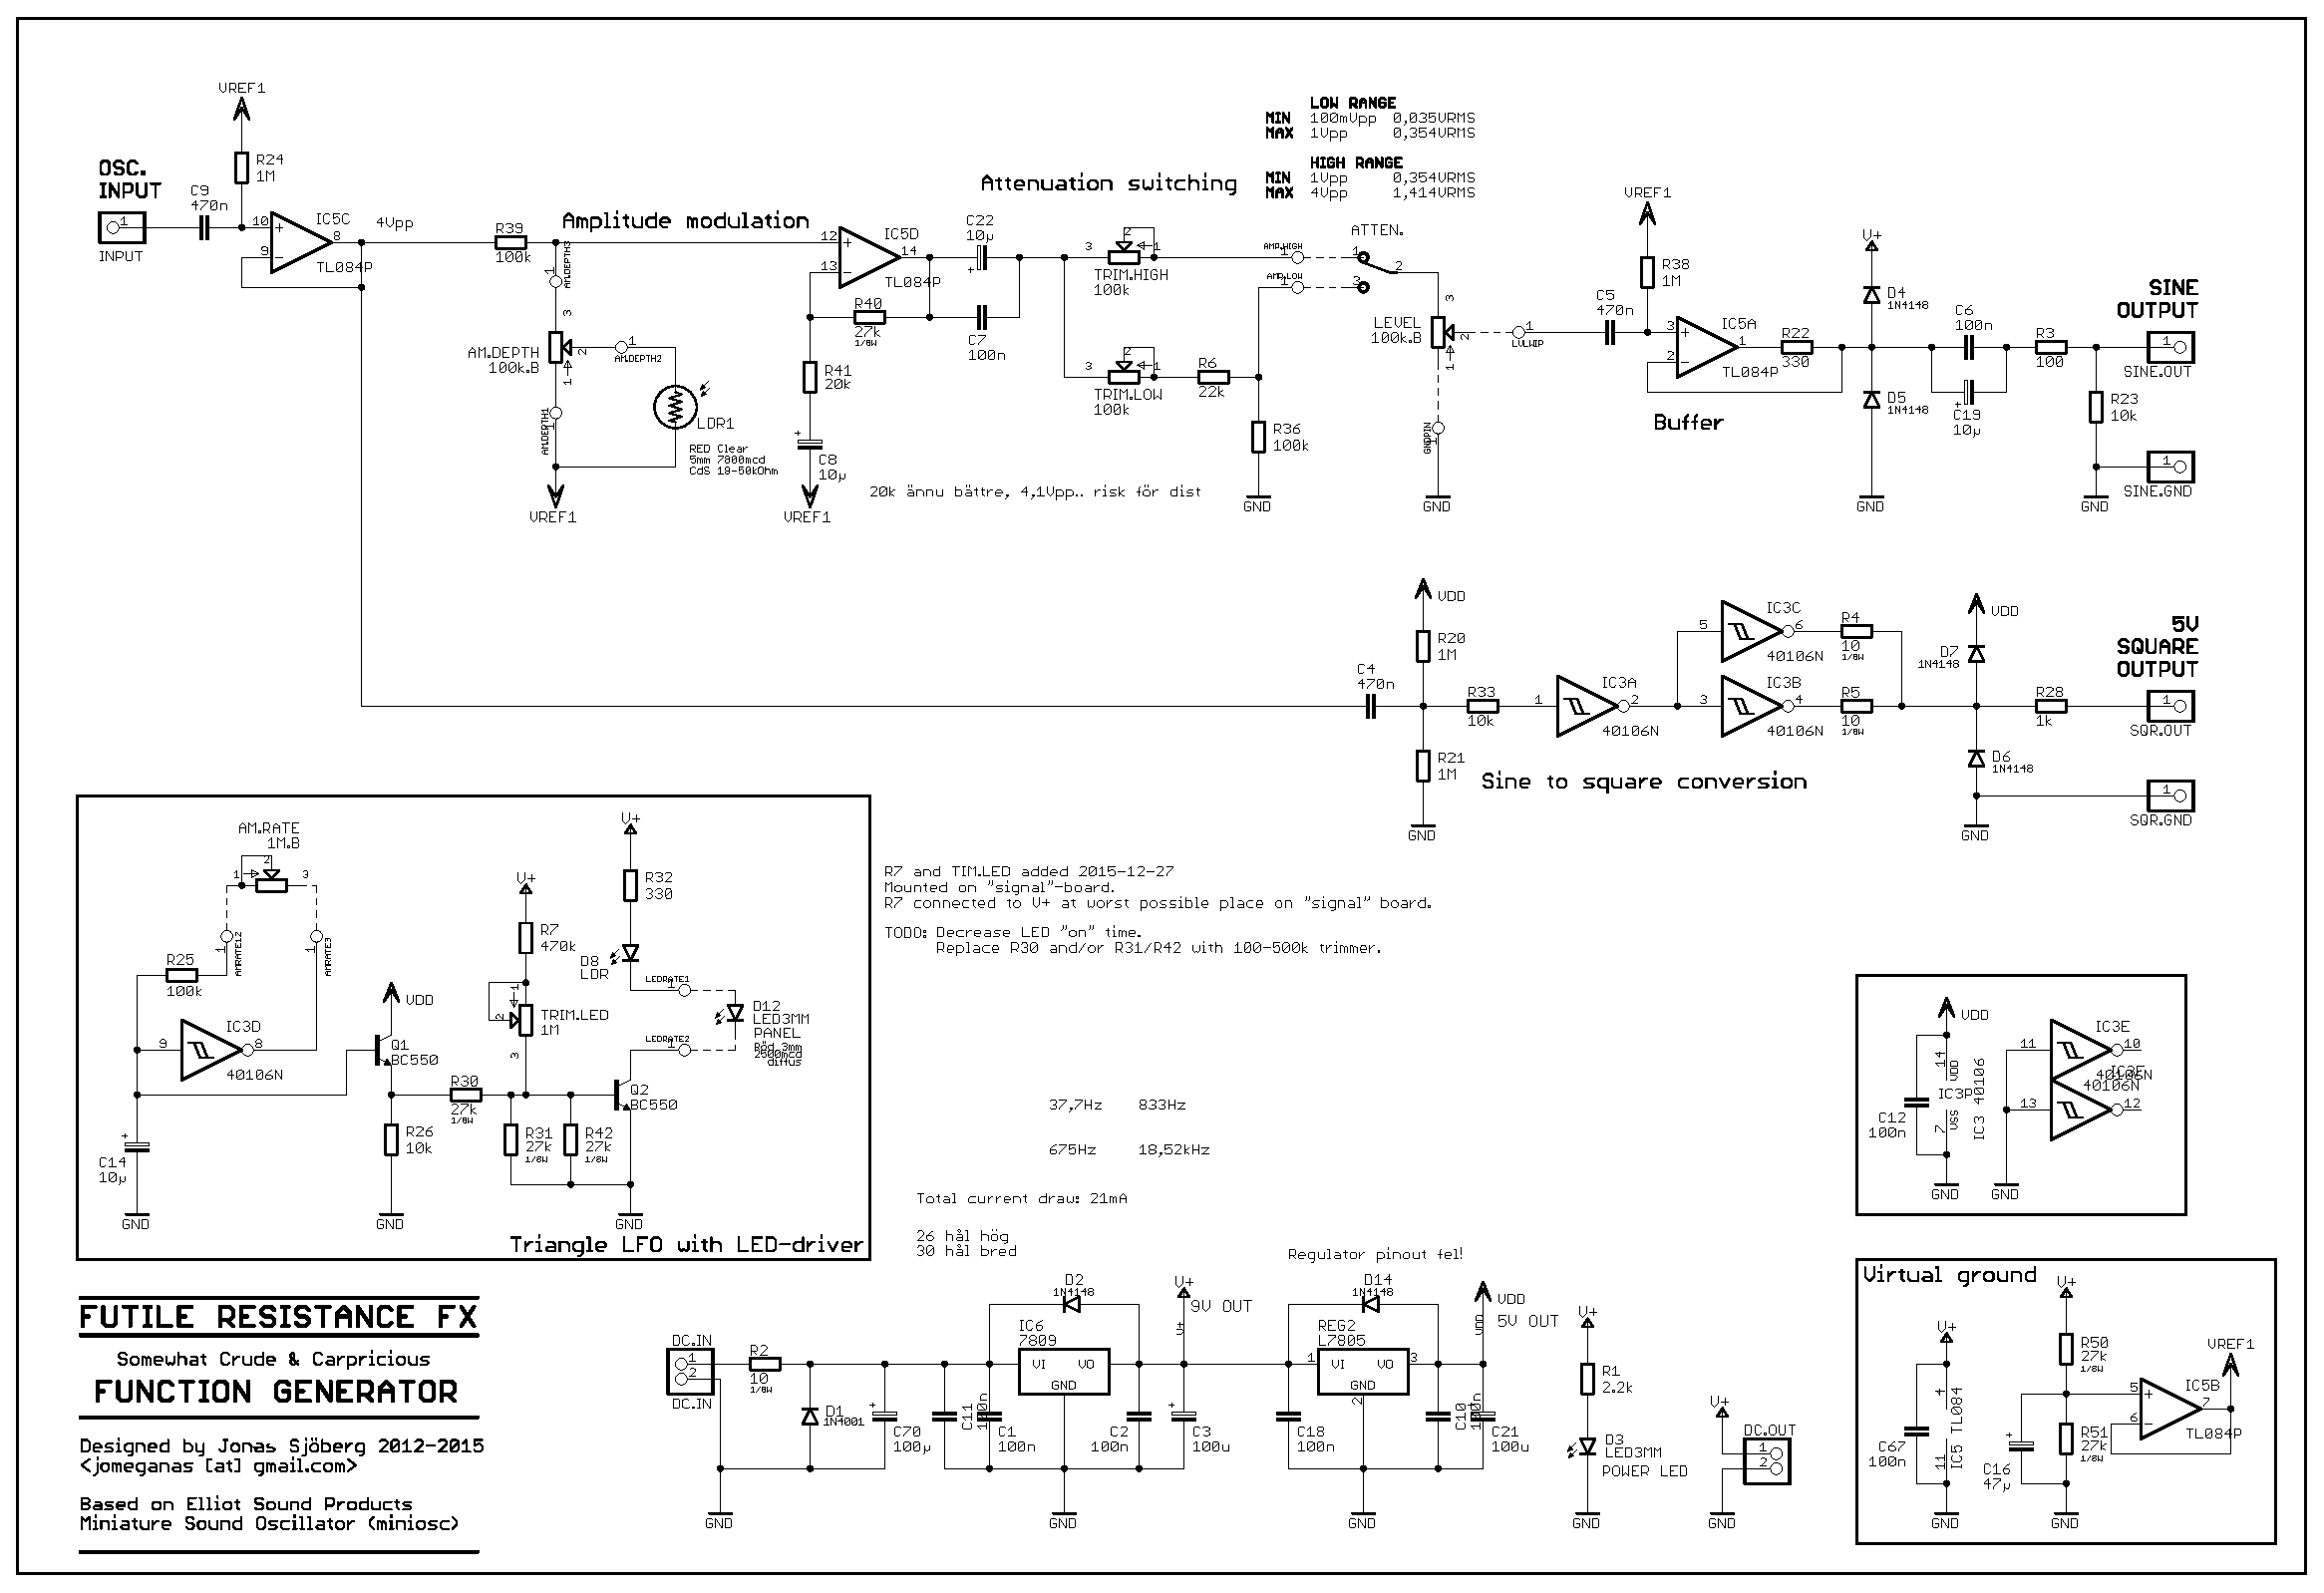
\includegraphics[width=\linewidth]{img/signal-generator_schematic-1}
 \caption{Kopplingsschema för signalgeneratorn som användes vid laborationen.}
\end{sidewaysfigure}

\begin{sidewaysfigure}[ht]\label{fig:siggen-schem-2}
 \centering
 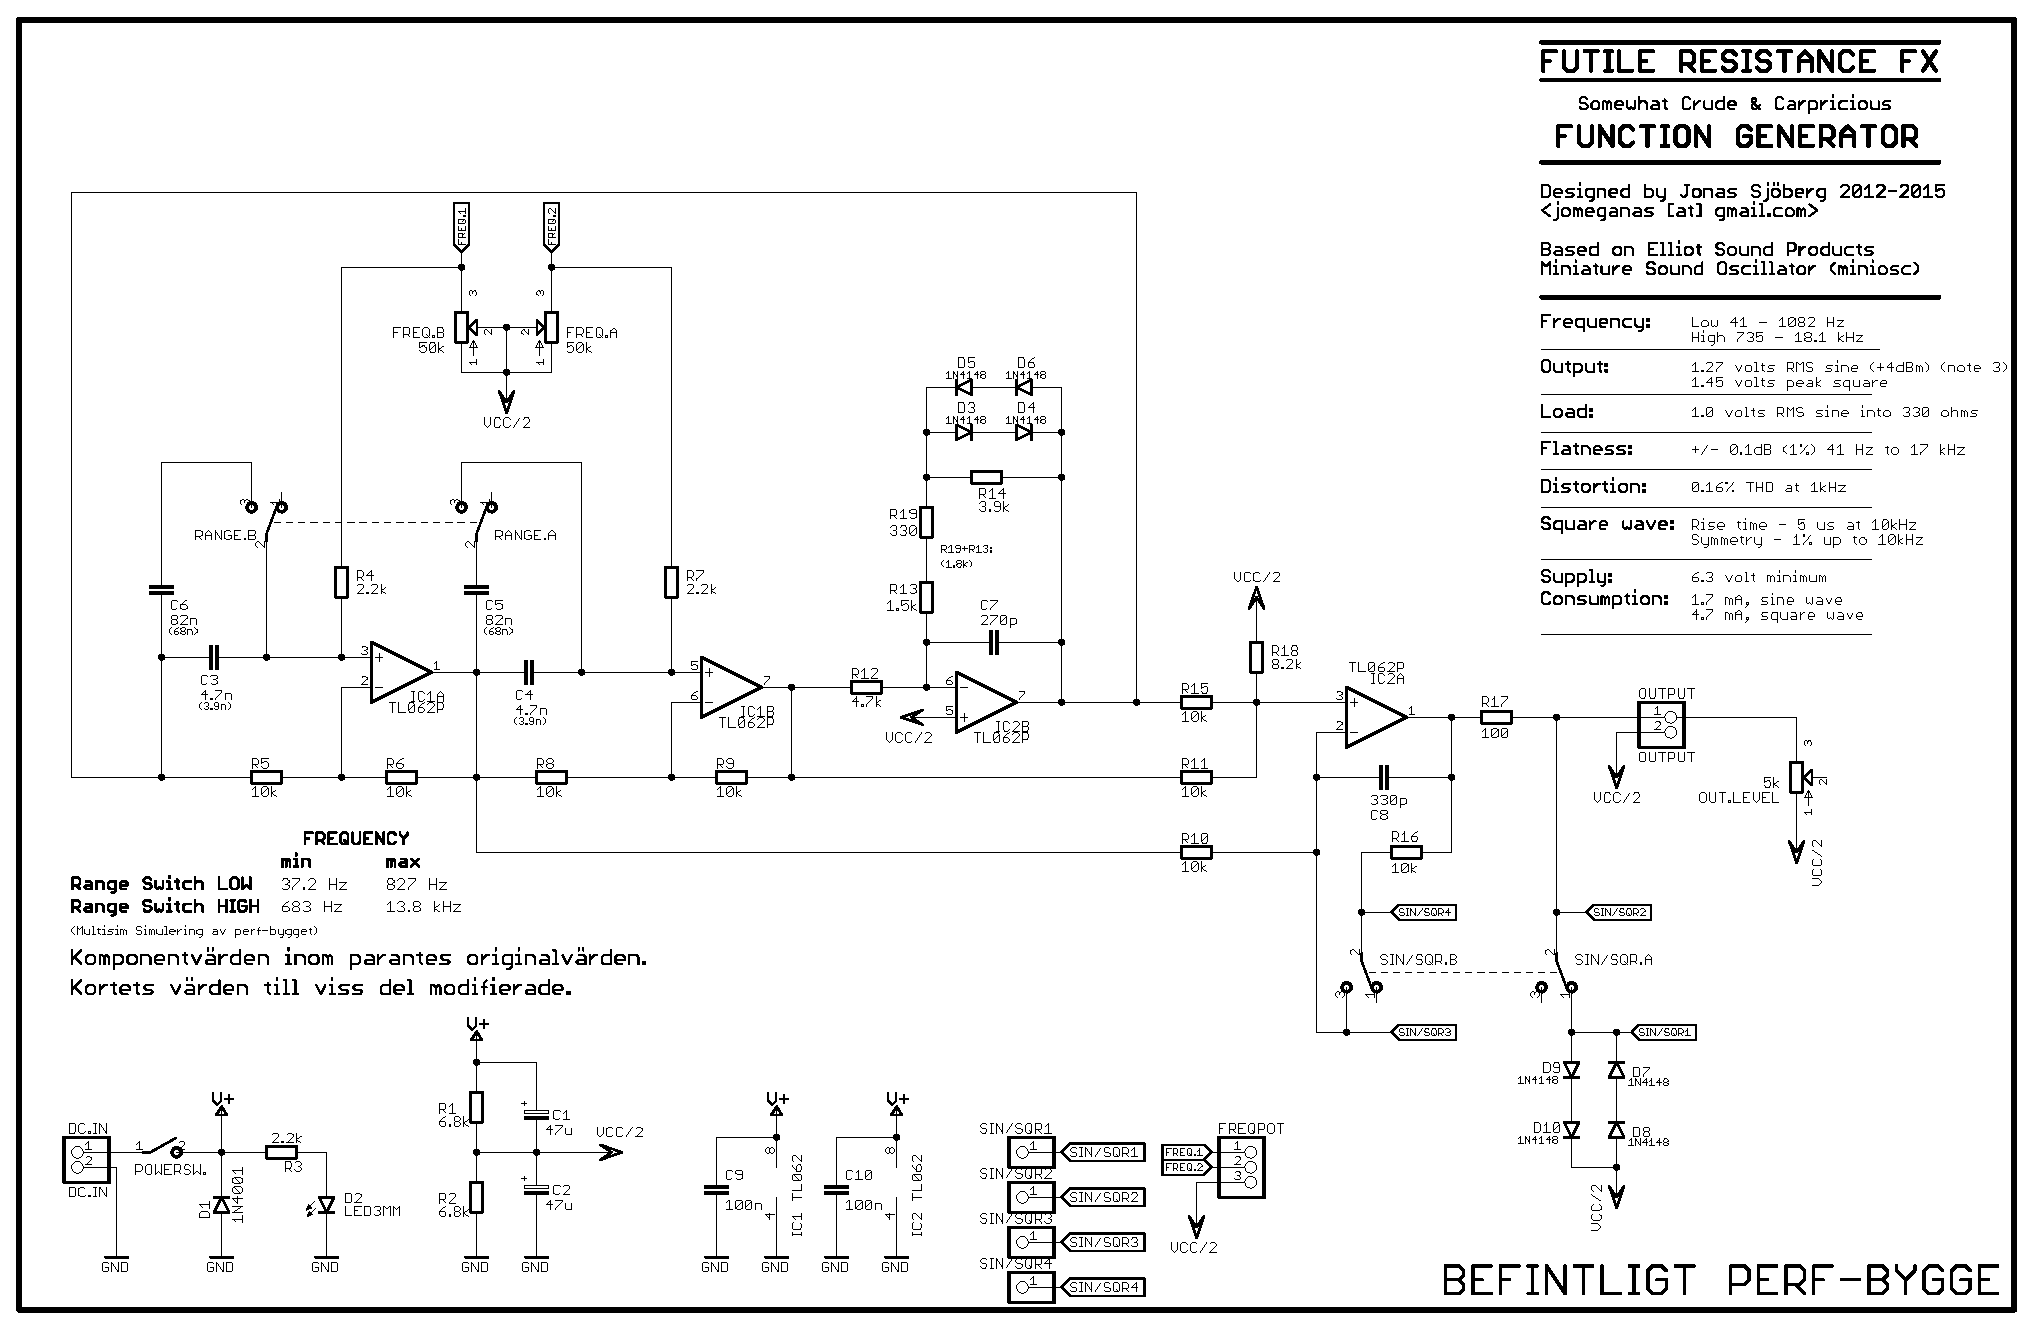
\includegraphics[width=\linewidth]{img/signal-generator_schematic-2}
 \caption{Kopplingsschema för signalgeneratorn som användes vid laborationen.
 Den här delen innehåller amplitudmodulering och trigger-utgången.}
\end{sidewaysfigure}


